\section{Introduction}
\label{sec:introdction}
Data exploration has gained lots of attentions over the last few years. The
main challenge is to support users with little prior knowledge, and no clear
objective. Some explorers need a preliminary impression of the data before
engaging into more structured tasks. Others are browsing in the hope to
discover new insights. Several authors have proposed tools to help data
exploration~\cite{abouzied2012dataplay, dimitriadou2014explore,
liarou2014dbtouch, sellam2013meet}. These systems offer some textual or
graphical interface, through which users can create, visualize and modify
selections of tuples quickly. Thus, explorers are engaged in a tight
trial-and-error loop, through which they discover their datasets. 

Data exploration systems rely on a crucial assumption: they suppose that if 
users see an interesting set of tuples (e.g., through tables or
visualizations), they will recognize it immediately, and think ``aha, this is
interesting''. This assumption may hold with small datasets, but it collapses
in higher dimensions. If the dataset contains  dozens, or hundreds of columns,
then which variables should the users inspect? Furthermore, which
\emph{combinations} of variables should they inspect? We cannot assume that
our data explorers know where to look.  Yet, studying each possibility in turn
can turn out to be a slow, tedious process. This beats the purpose of a data
exploration system.
%\begin{framed}
%    \everypar={{\setbox0=\lastbox}\everypar{}}
\textbf{How can we describe an arbitrary set of tuples when the
database contains more than a dozen columns?}
%\end{framed}

The straightforward approach is to use multidimensional visualizations such as
parallel coordinates or small multiples. Unfortunately, these methods tend to
show every possible aspect of the data, thus they do not scale well. For
instance, we would need at least 50 small multiples to visualize a dataset with
only 10 columns. Dimensionality reduction algorithms such as PCA or
ICA~\cite{guyon2003introduction} are also common, but they ignore the user's
selection, and hence may miss interesting combinations.  Besides, they rescale
and rotate the variables, causing their output to be harder to interpret.

In this paper we introduce our approach, \emph{multi-view subset
characterization}. The key idea is to detect subspaces inside which the user's
selection has an unusual distribution compared to the rest of the database.
These subspaces should be small, interpretable and non-redundant.  We
materialize this idea with Ziggy, a \emph{subset description engine}. For a
given subset of a database, Ziggy automatically generates a description of the
tuples with natural language and visualizations.  Thus, plugged on top of a
database engine, Ziggy can veritably simulate a conversation: the
user issues queries, and Ziggy replies in natural language. Our system can
process 10,000s tuples on dozens of variables within a second, and it can cope with
both numerical and nominal data, including missing values. To summarize:
\begin{itemize}
    \item We introduce and formalize the multi-view subset characterization problem.
    \item We describe Ziggy, a simple, efficient and robust system to describe
        selections of tuples in natural language
    \item We apply our system to real-life situations and benchmark it against
        state-of-the-art algorithms
\end{itemize}

Our paper is built as follows. In Sections~\ref{sec:genoverview}
and~\ref{sec:problem}, we present our problem. We instantiate this problem in
Section~\ref{sec:instantiation} and describe our algorithms in
Section~\ref{sec:algorithm}. We discuss how to validate our results and report
them in Sections~\ref{sec:validation} and~\ref{sec:reporting}. We describe how
to set parameters in Section~\ref{sec:parameters}. In
Sections~\ref{sec:usecase} and~\ref{sec:experiments}, we apply our solution to
real and synthetic data. Finally, we present related works and conclude in
Sections~\ref{sec:related-works} and \ref{sec:conclusions}.

\section{Overview}
\label{sec:genoverview}
\begin{figure}
  \centering
  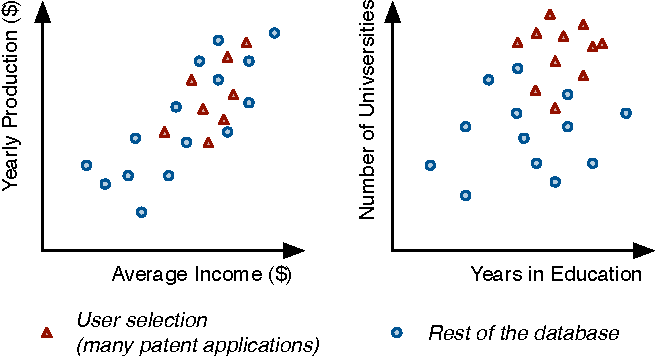
\includegraphics[width=\columnwidth]{Figures/Example}
  \caption{Two examples of subspaces for which the user's selection has an
  unusual distribution.}
  \label{pic:example}
\end{figure}
Let us introduce our problem through an example. A government analyst tries to
understand what demographic, social and economic factors lead to innovation.
More specifically, she is interested in patents: in which parts of the world do
individuals submit patents? What lessons can she learn? To answer this
question, our analyst collects several databases with regional statistics, and
loads them in her favorite business intelligence tool (possibly based on SQL or
spreadsheets). She selects the top 10\% regions for which many patents are
submitted, and ends up with an overwhelmingly large table, comprising a few
dozen tuples and hundreds of columns. How can we help her?
 
Our idea is to recommend views, which show how the selection of tuples differ
from the rest of the database. Figure~\ref{pic:example} shows two of these
views. We see that on the columns \texttt{Average Income} and \texttt{Yearly
Production}, the tuples are gathered in top-right corner of the chart. The
effect is even stronger on the second plot, which shows the variables
\texttt{Years in Education} and \texttt{Number of Universities}. Observe that
these views have a purposely low dimensionality. Our aim is not to show
\emph{all} the variables on which the selection has an impact. Instead, we
recommend a few small, non redundant groups, each illustrating one
characteristic of the tuples. We call this approach \emph{multi-view subset
characterization}.

Once we detected the views, we can depict them with visualizations as in
Figure~\ref{pic:example}. The merits of this approach is hardly disputable, in
particular compared to tables. And yet, analyzing charts takes time and
training. Not all effects are perceptible, in particular when the views
contain three dimensions or more. Lastly, charts are simply not accessible to
visually impaired users. To address these problems, we propose to exploit a
different communication channel: we generate natural language descriptions of
the views. For instance, we could describe the views pictured in
Figure~\ref{pic:example} as follows:
\begin{quotation}
    On the columns~\texttt{Average Income} and \texttt{Year\-ly Production},
    your selection has a high value and high concentration. The effect is
    similar and stronger on \texttt{Years in Education} and \texttt{Number of
    Universities}.
\end{quotation}
Note that we \emph{describe} the data, but we do not \emph{interpret} it. The
latter problem is much harder, and we claim in no way to have solved it. We
will however dare to issue simple ma\-gni\-tude judgments, such as ``this
effect is particularly strong'', using conservative, transparent hand-written
rules.


\section{General problem statement}
\label{sec:problem}
Let us now formalize the multi-view characterization problem. We represent our
database with a matrix $\rb{D}$, with $M$ columns and $N$ rows.  We model 
each tuples by an iid. random vector  $\rb{x}_n = (x^1_n, \dots, x^M_n)^\top$,
and each column by  $\rb{x}^{m}= (x^m_1, \dots, x^m_N)^\top$.

Let the submatrix $\rb{V}  = [\rb{x}^1, \dots, \rb{x}^V]$ describe a view
(i.e., subspace, or set of columns). We split this view in two:  ${\rb{V}}_t$
contains the tuples in the selection, ${\rb{V}}_{\overline{t}}$ the remainder,
as shown below:
\begin{figure}[h!]
  \centering
  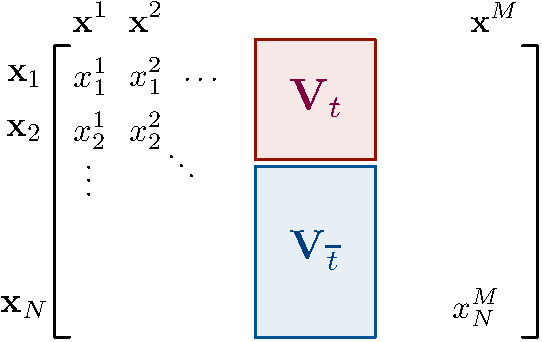
\includegraphics[width=0.5\columnwidth]{Figures/Notations}
%  \caption{Our notations.}
  \label{pic:notations}
\end{figure}


To measure how much $\rb{V}_t$ and ${\rb{V}}_{\overline{t}}$ differ, we compare
the empirical probability distribution of their rows. If these distributions
differ, then the view exhibits some ``peculiarity'' of the data.  Therefore,
$\rb{V}$ is likely to be informative. We measure this difference with a
\textbf{mass dissimilarity measure} $\mf{D}(\rb{V}_t, \rb{V}_{\nott})$.  This
function returns 0 if the tuples come from from the same distribution, it grows
otherwise. The statistics literature contains several candidates, for example
estimators the Kullback-Leibler Divergence~\cite{wasserman2013all}. We will
present our own function in the following section.

We can already propose a first, naive, formulation of our problem:
\begin{problem}
    Consider a distribution dissimilarity function $\mf{D}$ and two integers
    $K$ and $D$. Find the top $K$ distinct views $\rb{V}^i$ with at most $D$
    dimensions which maximize $ \mf{D}\big( \rb{V}^i_t ;
    \rb{V}^i_{\overline{t}} \big)$ (ignoring column permutations).
\end{problem}

This approach is simple, but it yields redundancy: a small number of good
columns may dominate the results and appear in all $K$ views. In a data
exploration scenario, users may value \emph{diversity}, even if the views are
sub-optimal. To enforce this requirement, we introduce a penalty factor in our
objective function.
\begin{table*}[t!]
    \centering
  \rowcolors{2}{gray!25}{white}
    \begin{tabular}{ccccp{9cm}}
      \hline
    \rowcolor{gray!50}
      Property & Type 1 & Type 2 & Zig-Component & Comments\\
      \hline
      Mean & Contin.  & - &
      $  \mf{z}_m^{\bf{d}}  = (\bar{\bf{d}}_t - \bar{\bf{d}}_{\nott}) / s_{\overline{t}}$ & 
      Known as Glass' $\Delta$~\cite{hedges2014statistical}\\
      Stand. Dev.& Contin.  & - &
      $ \mf{z}_{\sigma}^{\bf{d}}=(s_t-s_{\nott})/s_{\overline{t}}$ & \\
      Frequencies & Discrete & - & 
      $\mf{z}_\chi ^{\bf{d}}= \sqrt{\chi^2}$ &
      Based on Pearson's $\chi^2$ goodness-of-fit test~\cite{wasserman2013all}\\
      Dependence & Contin. & Contin. & $\mf{z}_r^{\bf{d}, \bf{d}'}  = r_t - r_{\nott} $ & 
      $r_t$is the correlation coefficient between $\bf{d}_t$ and  $\bf{d}'_t$\newline
      $r_{\nott}$ is the correlation coefficient between $\bf{d}_{\nott}$ and
      $\bf{d}'_{\nott}$~\cite{wasserman2013all}\\
     Dependence  & Discrete & Both & $ \mf{z}_V^{\bf{d}, \bf{d}'} = V_t - V_{\nott} $ &
           $V_t$ is Cram\'er's V coefficient between $\bf{d}_t$ and  $\bf{d}'_t$ \newline
           $V_{\nott}$ is Cram\'er's V coefficient between $\bf{d}_{\nott}$ and
           $\bf{d}'_{\nott}$~\cite{cohen1977statistical} \\ 
      \hline
    \end{tabular}
    \caption{Our choice of Zig-Components for different data types. Each
        component describes a difference, to be evaluated for either each
        column $\bf{d}$ or each couple of columns $\bf{d}, \bf{d}'$ in the
        view. The notations $\bar{\bf{d}}$ and $s$ respectively represent the
        sample mean and sample standard deviation. In the mixed-types case, we
        discretize the continuous column with equi-width binning.}
    \label{tab:dissim}
\end{table*}

Measuring redundancy between column is not straightforward, as this notion is
partially subjective. In our model, we exploit statistical dependency: if two
sets of columns are tightly correlated, then there is a high chance that they
describe the same property of the ``real world''.  Oppositely, if they are
independent, then they probably convey different types of information. From
this observation, we introduce a new version of our problem: we seek views
which maximize the distance statistic, while minimizing inter-view dependency.
We define this problem in a recursive way:
\begin{problem}
    Suppose that we have already detected $i-1$ views ($i > 1$,
    $\rb{V}^{0} = \emptyset$). We obtain $\rb{V}^{1..i-1} = [\rb{V}^1, \ldots,
    \rb{V}^{i-1}]$ by concatenating these views. Let $\mf{S}$ describe a
    statistical dependency measure. Given a positive real $\lambda$, find the
    view $\rb{V}^{i}$ with at most $D$ columns which maximizes:
        \begin{equation}
            \label{prob1}
            \mf{D}\big( \rb{V}^{i}_t  ; \rb{V}^{i}_{\overline{t}} \big) - 
            \lambda \cdot \mf{S} ( \rb{V}^{i} ; \rb{V}^{1..i-1})
        \end{equation}
\end{problem}
Statistics textbooks offer many options to instantiate the dependency measure
$\mf{S}$. Well established examples are multivariate variants of the
correlation coefficient, or the mutual information~\cite{wasserman2013all}.
Here again, we will present our own function in Section~\ref{sec:dependency}.

In Equation~\ref{prob1}, the parameter $\lambda$ controls the trade-off between
mass distance and view diversity: a high value enforces that that the view are
diverse, while a low value expresses our preference for maximizing $\mf{D}(
\rb{V}^{i}_t  ; \rb{V}^{i}_{\overline{t}})$. In practice, this parameter is
not convenient because it has no intuitive scale. For some $L$, an
equivalent way to express our problem is the following:
\begin{equation}
    \label{prob2}
    \begin{aligned}
        & \text{Argmax}_{\rb{V}^{i}} 
            & \mf{D}\big( \rb{V}^{i}_t  ; \rb{V}^{i}_{\overline{t}} \big)\\
        & \text{s.t.} 
        &\mf{S} ( \rb{V}^{i} ; \rb{V}^{1..i-1}) & < L\\ 
    \end{aligned}
\end{equation}
Equation~\ref{prob1} in the Lagrangian of Equation~\ref{prob2}, up to a
negligible additive constant. We prefer this form because the trade-off
parameter $L$ has the same scale as $\mf{S} ( \rb{V}^{i} ; \rb{V}^{1..i-1}) $.
For example, if we instantiate $\mf{S}$ with correlation, then $L$ will simply
describe the maximal acceptable correlation between $\rb{V}^{i}$ and
$\rb{V}^{1..i-1}$.

\section{Instantiation: Meet Ziggy}
\label{sec:instantiation}
We now instantiate the dissimilarity measure $\mf{D}$ and redundancy measure
$\mf{S}$. 

\subsection{Explainable Mass Dissimilarity}
\label{sec:explain}
\begin{figure}
  \centering
  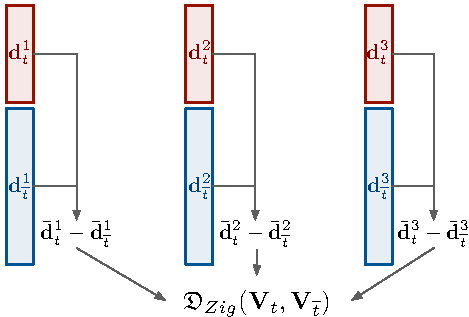
\includegraphics[width=0.7\columnwidth]{Figures/Zig-Dissim}
  \caption{Illustration of Ziggy's Dissimilarity.}
  \label{pic:zigdis}
\end{figure}

Let us begin with the dissimilarity~$\mf{D}$. As mentioned previously, we could
borrow any general divergence measure from the statistics literature, such as
the KL-divergence. However, these measurements operate as ``black boxes'': they
describe the intensity of the differences, but they do not explain how the
tuples differ. Our approach is diametrically opposed: we introduce the
\textbf{Zig-Dissimilarity} $\mf{D}_{Zig}$, a completely \emph{explainable}
mass dissimilarity measure.

The idea behind our dissimilarity measure is to compute several simple,
interpretable indicators of difference, called \textbf{Zig-Components}, and
aggregate them in a single composite score, the Zig-Dissimilarity.  Consider
for instance two sets of tuples $\rb{V}_t$ and $\rb{V}_{\nott}$ with $V$
columns. If these subsets have the same average for every column, then they
probably come from the same distribution. Oppositely, if the averages are
different, then they probably come from different distributions. From this
observation, we can build an elementary dissimilarity measure: for each column
$\bf{d}$, we compute the differences between the means $\bar{\bf{d}}_t -
\bar{\bf{d}}_{\nott}$, as shown in Figure~\ref{pic:zigdis}. These are our
Zig-Components. We could add more components by measuring other properties,
such as the difference between the variances. To obtain the  Zig-Dissimilarity,
we aggregate all these components into one composite indicator.
\begin{definition}
    A Zig-Component is a function $\mf{z} : \rb{V}\times\rb{V} \to \mathbb{R}$
    which describes one difference between two sets of tuples. If the tuples
    are similar, then $\mf{z}(\rb{V}_t, \rb{V}_{\nott}) = 0$. If not,
    the magnitude of $\mf{z}(\rb{V}_t, \rb{V}_{\nott})$ varies with the strength
    of the difference.
\end{definition}
For the sake of presentation, we  abbreviate $\mf{z}(\rb{V}_t, \rb{V}_{\nott})$
as~$\mf{z}$.

In our implementation, we combined five types of Zig-Com\-po\-nents, summarized
in Table~\ref{tab:dissim}.  A few of them come from the statistics literature,
where they are referred to as \emph{effect sizes}~\cite{cohen1977statistical,
hedges2014statistical}.  We chose these indicators because they have intuitive
interpretations, as well as known asymptotic properties (we will use those
Section~\ref{sec:validation}).  A majority, but not all of them are normalized
and vary between -1 and 1. None of these functions are symmetric, and most of
them change sign according to the direction of the underlying effect.

Observe that Ziggy computes univariate, but also bivariate components: in this
case it compares columns by pairs. Our motivation is to check which
correlations are present in $\bf{V}_t$ and not in $\rb{V}_{\nott}$, or more
generally which correlations are either strengthened or weakened across the
subsets. In the discrete case, we substitute the correlation coefficient by
Cram\'er' s V.  This function also measures the associations between two
variables, and it varies similarly between 0 and 1~\cite{cohen1977statistical}.
Its value is $\sqrt{\chi^2/(N(\min(|\bf{d}_t|,|\bf{d}_{\nott}|) - 1))}$, where
$\chi^2$ is Pearson's $\chi^2$ statistic, and $|\bf{d}_t|,|\bf{d}_{\nott}|$ are
the number of distinct values in $\bf{d}_t$ and $\bf{d}_{\nott}$ respectively.

Once we computed the Zig-Components $\mf{z}_1, \ldots, \mf{z}_Z$, we obtain the
Zig-Dissimilarity as follows. First, we compute the absolute values
$|\mf{z}_1|, \ldots, |\mf{z}_Z|$ for each component. We then normalize the
values across components of same type. We obtain a set of intermediary scores
$z_1, \ldots, z_Z$. We aggregate these scores with a weighted sum.
These operations give us one scalar indicator, which summarizes the magnitude
of all the differences.

\begin{definition}
    Let $z_1, \ldots, z_Z$ represent a set of normalized absolute values of
    zig-components, and $w_1, \ldots, w_Z$ a set of user-defined weights.  We
    define the Zig-Dissimilarity as follows: 
    \begin{equation}
        \mf{D}_{Zig}(\rb{V}_t, \rb{V}_{\nott}) 
        \equiv \sum_{k \in [1, Z]} w_k \cdot z_k(\rb{V_t}, \rb{V}_{\nott})
    \end{equation}
\end{definition}
We insist that the Zig-Components must be normalized before the aggregation.
In the general case, we cannot assume that the scores are commensurate.

The aim of the weights $w_k$ is to balance the effects across column types. For
instance, we measure two components for the numerical columns, and only one for
categorical data.  Thus, we set $w_k = 1/2$ for the former and $w_k = 1$
for the latter.  These parameters also let users express their preferences: for
example, a novice user may value one-dimension Zig-Components over those based
on correlation.

Table~\ref{tab:dissim} reports univariate, then bivariate Zig-Components.  In
principle, we could test differences in spaces with more dimensions.  We chose
not to do so, for two reasons. First, relationships in three dimensions or more
are harder to convey and understand in natural language.  Second, the number of
relationships to be inspected grows exponentially with the dimensionality of
the Zig-Component. This hurts Ziggy's runtime, and leads to much longer
outputs. We will show in Section~\ref{sec:experiments} that this restriction
has little practical effect on the Ziggy's views.


\subsection{Dependency Measure}
\label{sec:dependency}
\begin{figure}
  \centering
  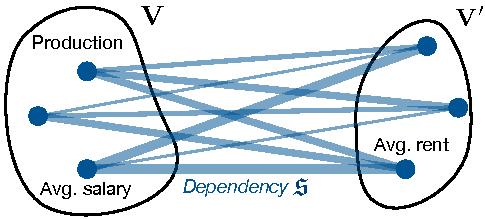
\includegraphics[width=0.6\columnwidth]{Figures/Redundancy}
  \caption{Illustration of Ziggy's redundancy measure. Vertices represent
  column, edges represent pairwise dependency.}
  \label{pic:redundanct}
\end{figure}
We now present two instantiations for the measure of redundancy,
$\mf{S}_{hard}$ and $\mf{S}_{soft}$.  Both measures are a variant of the same
principle, and we will refer to them collectively as the Zig-Dissimilarity
$\mf{S}_{Zig}$. Here again, the main idea is to aggregate several simple
interpretable indicators, such as those that users can find in statistics
textbooks.

Let  $\rb{V}$ and $\rb{V}'$ represent two views. We compute the Zig-Dependency
in two steps. First, we compute the pairwise dependency $\mf{s}(\rb{d},
\rb{d}')$ between every column $\rb{d}$ of  $\rb{V}$ and every column $\rb{d}'$
of $\rb{V}'$, as shown in Figure~\ref{pic:redundanct}. The measure $\mf{s}$ is
a convenience function, which allows us to combine different types of
variables:
\begin{equation}
    \mf{s}(\rb{d}, \rb{d}')= \begin{cases}
        r(\rb{d}, \rb{d}')\ \text{if $\bf{d}, \bf{d}'$ are continuous (correlation)}\\
        V(\rb{d}, \rb{d}')\ \text{otherwise (Cram\'er's V, cf.
        Sec.~\ref{sec:explain})}
         \end{cases}
\end{equation}
During the second step, we aggregate these dependencies. The function
$\mf{S}_{hard}$ utilizes the maximum, while $\mf{S}_{soft}$ uses the mean:
\begin{gather}
    \mf{S}_{hard}(\rb{V}, \rb{V}') = \max_{d \in \rb{V}, d' \in \rb{V}'} |\mf{s}(d, d')|
    \label{eq:hard}\\
    \mf{S}_{soft}(\rb{V}, \rb{V}') = 
    \frac{\sum_{d \in \rb{V}, d' \in \rb{V}'} |\mf{s}(d, d')|}
    {V \cdot V'}
    \label{eq:soft}
\end{gather}
Both functions $\mf{S}_{soft}$ and $\mf{S}_{hard}$ vary between 0 and 1, 0
indicating no dependency. The crucial difference lies in how they treat
overlap. If one column is present in both $\rb{V}$ and $\rb{V}'$, then
$\mf{S}_{hard}$ is at its maximal value 1, regardless of the other columns in
the views. It is not necessarily so for $\mf{S}_{soft}$. Thus
$\mf{S}_{hard}$ leads to less redundancy, while $\mf{S}_{soft}$ is more
flexible. We will demonstrate these effect in our Experiments section.

Finally, observe that our choice for $\mf{S}$ is computationally efficient: we
get the pairwise correlations ``for free'', because we need to compute them
anyway to obtain the Zig-Components $\mf{z}_{\chi}$ and $\mf{z}_r$.

\section{Algorithms To Detect Views}
\label{sec:algorithm}

We introduced a mass dissimilarity measure $\mf{D}_{Zig}$ and a view dependency
measure $\mf{S}_{Zig}$. We now discuss how to maximize the former while
constraining the latter, as exposed in Equation~\ref{prob2}.

\subsection{Overview}
\label{sec:overview}

\begin{figure}
  \centering
  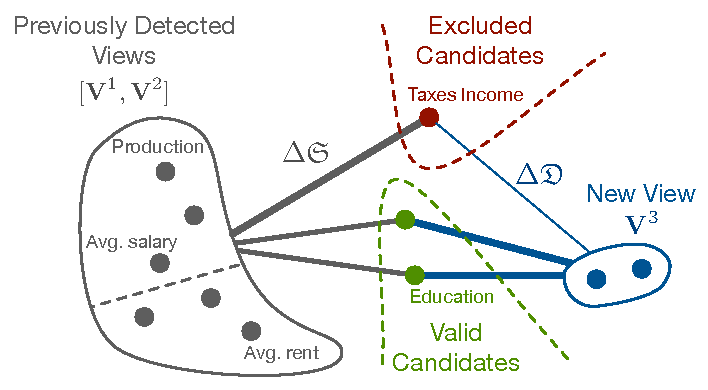
\includegraphics[width=0.8\columnwidth]{Figures/Greedy}
  \caption{Illustration of Ziggy's greedy view composition algorithm, with
  $i=3$ and $D=3$. The grey edges represent the
  amount of redundancy added by each candidate. The blue edges represent the
  amount of dissimilarity added by each candidate.}
  \label{pic:greedy}
\end{figure}
\begin{algorithm}[t!]
\caption{View Construction}
\label{algo:view_search}
\begin{algorithmic}
    \Function{DetectViews}{$K$, $D$, $L$}
    \For{$k \in [1,K]$}
        \State $\text{Cand} \gets \{\rb{x}^1, \ldots, \rb{x}^M\}$
        \State $\text{Red.Gains} \gets 
            \{\Delta\mf{S}(\rb{d}, \rb{V}^{1..k}), \text{~for~} \rb{d} \in \text{Cand}\}$
         \State $\text{Cand} \gets 
            \{\rb{d} \text{~where~not~Red.Gains}(\rb{d}) > L \}$
        \State $\text{Dis.Gains} \gets 
        \{\Delta\mf{D}(\rb{d}, \rb{d}'), \text{~for~} \rb{d},\rb{d}' \in \text{Cand}\}$
        \State $\rb{V}^k \gets \rb{V}^k \cup \{\text{argmax}_{\bf{d}, \bf{d}'}\ \text{Dis.Gains}\}$
        \For {$d \in [3, D]$}
            \State $\text{Cand} \gets \{\rb{x}^1, \ldots, \rb{x}^M\}
                \setminus \rb{V}^k$
            \State $\text{Red.Gains} \gets 
                \{\Delta\mf{S}(\rb{d}, \rb{V}^{1..k}), \text{~for~} \rb{d} \in \text{Cand}\}$
             \State $\text{Cand} \gets 
                \{\rb{d} \text{~where~not~Red.Gains}(\rb{d}) > L \}$
            \State $\text{Dis.Gains} \gets 
                \{\Delta\mf{D}(\rb{d}, \rb{V}^{k}), \text{~for~} \rb{d} \in \text{Cand}\}$
            \State $\rb{V}^k \gets \rb{V}^k \cup \{\text{argmax}_{\bf{d}}\ \text{Dis.Gains}\}$
        \EndFor
    \EndFor
    \EndFunction
\end{algorithmic}
\end{algorithm}

Once the user has provided a selection of tuples, Ziggy performs two steps.
First, it computes the Zig-Components, for each column and each pair of columns
in the database. Then, it composes the views greedily: it picks the
co\-lumns associated with the highest components one by one, while ensuring
that the dependency threshold $L$ is not breached.

The first step is straightforwards, but it is also by far the most time
consuming. We discuss in Section~\ref{sec:optimization} how to optimize it.
During the second step Ziggy creates the views by adding columns in a
best-first fashion.  Figure~\ref{pic:greedy} illustrates this approach. Suppose
that Ziggy has previously obtained two views, $\rb{V}^1$ and $\rb{V}^2$, and it
is currently building a third one, $\rb{V}^3$. For each column in $\rb{V}
\setminus \rb{V}^3 $, our algorithm computes two scores: the gain of
dissimilarity $\Delta\mf{D}$ induced by adding the candidate to $\rb{V}^3$, and
the gain of redundancy~$\Delta\mf{S}$ induced by the same. Ziggy excludes the
columns which exceed the redundancy capacity, e.g., those for which
$\mf{S}([\rb{V}^1, \rb{V}^2], \rb{V}^3) + \Delta\mf{S} > L$. It then detects
the best candidate among those that remain and adds it to the view. It repeats the
process until either the maximal number of columns $D$ is met, or there are no
more eligible columns. We present the pseudo-code in
Algorithm~\ref{algo:view_search}.

To compute $\Delta\mf{S}$, we apply Equations~\ref{eq:hard} and~\ref{eq:soft}
directly. Computing $\Delta\mf{D}$ requires more care, because each column is
involved in several Zig-Com\-po\-nents, and the bivariate components
depend on the current state of the algorithm.  Suppose for instance that we are
building a view $\rb{V}^{i}$, and we wish to compute $\Delta\mf{D}$ for a given
candidate $\bf{d}$.  In our implementation, if $\bf{d}$ contains numeric
values, then it is associated with at least two components: the difference
between the means $\mf{z}_\mu$, and the difference between the standard
deviations $\mf{z}_\sigma$. We obtain those from the first step of the
algorithm.  But we must also account for the difference between dependencies,
for all the columns already included in $\rb{V}^{i}$. Thus, if $z$ describes
the normalized absolute value of a Zig-Component $\mf{z}$, and if
$\rb{V}^{i}_{num}$ and $\rb{V}^{i}_{cat}$ respectively represent the numerical
and categorical variables of $\rb{V}^{i}$ the final score is:
%\begin{equation}
    \begin{multline}
\Delta\mf{D} = 
z_\mu^{\bf{d}}+ z_\sigma^{\bf{d}} +
\sum_{\rb{d}' \in \rb{V}^i_{num}} z_r^{\rb{d}, \rb{d}'}
+ \sum_{d' \in \rb{V}^i_{cat}} z_V^{\rb{d}, \rb{d}'}
\end{multline}
%\end{equation}
The last two terms of the equation depends on the current state of $ \rb{V}^i$.
Therefore we must update $\Delta\mf{D}$ after each step.

If we use the redundancy measure $\mf{S}_{hard}$, then we can avoid computing $
\Delta\mf{S}$ altogether: Ziggy can discard the redundant candidates before it
starts building the view.  Consider a candidate column $d$, and let
$\rb{V}^{1..i-1}$ describe the union of all previously built views. If
$\mf{S}_{hard} (\rb{V}^{1..i-1}, d) > L$, then the column is not exploitable:
adding it to the current view $\rb{V}^{i}$ will breach the threshold,
regardless of $\rb{V}^{i}$'s current state.  Conversely, if we have
$\mf{S}_{hard}(\rb{V}^{1..i-1}, d) < L$, then candidate is ``safe'', it will
never breach the dependency threshold.  Thus Ziggy, builds the
view in two separate steps: first it eliminates the redundant columns (i.e.,
those for which $\mf{S}_{hard} (\rb{V}^{1..i-1}, d) > L$), then it selects the
top $D$ candidates. 

Finally, observe that our greedy algorithm is not exact, but it runs
in~$\mathcal{O}(KMD)$. Thanks to this heuristic, we avoid an exhaustive search
of $\binom{M}{D}$ possible possible view combinations, which would lead to an
unpractical $\mathcal{O}(KM^D)$ runtime.


\begin{table*}[t!]
    \centering
  \rowcolors{2}{gray!25}{white}
    \begin{tabular}{c c c c p{8cm}}
    \rowcolor{gray!50}
      \hline
      Property & Type 1 & Type 2 & Test Statistic & Comment\\
      \hline
      Mean & Contin.  & - & $(\bar{\bf{d}}_t - \bar{\bf{d}}_{\nott})/s_{\bar{\bf{d}}_t - \bar{\bf{d}}_{\nott}}$ &
        Wald test~\cite{wasserman2013all}  \\
        Stand. Dev.& Contin.  & - & $s_t / s_{\nott}$ &
        F-test~\cite{cohen1977statistical} \\
        Frequencies & Discrete & - & $\chi^2$ & Pearson's $\chi^2$
        test~\cite{wasserman2013all}\\
      Dependence  & Contin. & Contin & $(Z_t - 
      Z_{\nott})/s_{Z_t - Z_{\nott}}$ & $Z$ is the Fisher
      Z-transformation of the correlation coefficient $r$ between $\bf{d}$ and
      $\bf{d}'$~\cite{fisher1915frequency}\\
      Dependence  & Contin. & Both &  $(V_t - V_{\nott})/s_{V_t-V_{\nott}}$ & $V$ is
      Cram\'er's V between $\bf{d}$ and $\bf{d}'$. We obtain its distribution with Fisher's
      Normal approximation of $\sqrt{\chi^2}$~\cite{patel1996handbook}.\\ 
      \hline
    \end{tabular}
\caption{Our choice of tests, corresponding to each Zig-Component. We use the
same notations as in Table~\ref{tab:dissim}.}
    \label{tab:tests}
\end{table*}
\begin{figure}[t!]
    \centering
    \begin{subfigure}[b]{\columnwidth}
    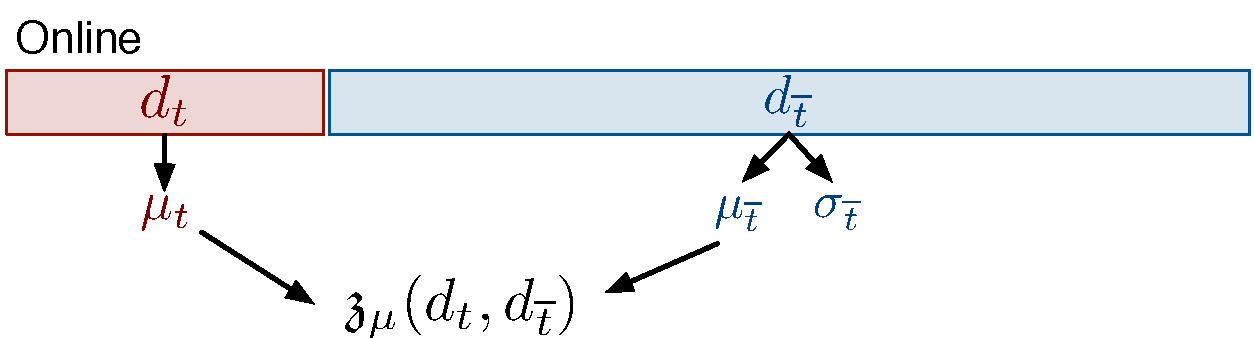
\includegraphics[width=\textwidth]{Figures/Staging}
    \caption{Computing $\mf{z}_\mu$ without staging.}
    \label{pic:withoutstag}
    \end{subfigure}

    \begin{subfigure}[b]{\columnwidth}
        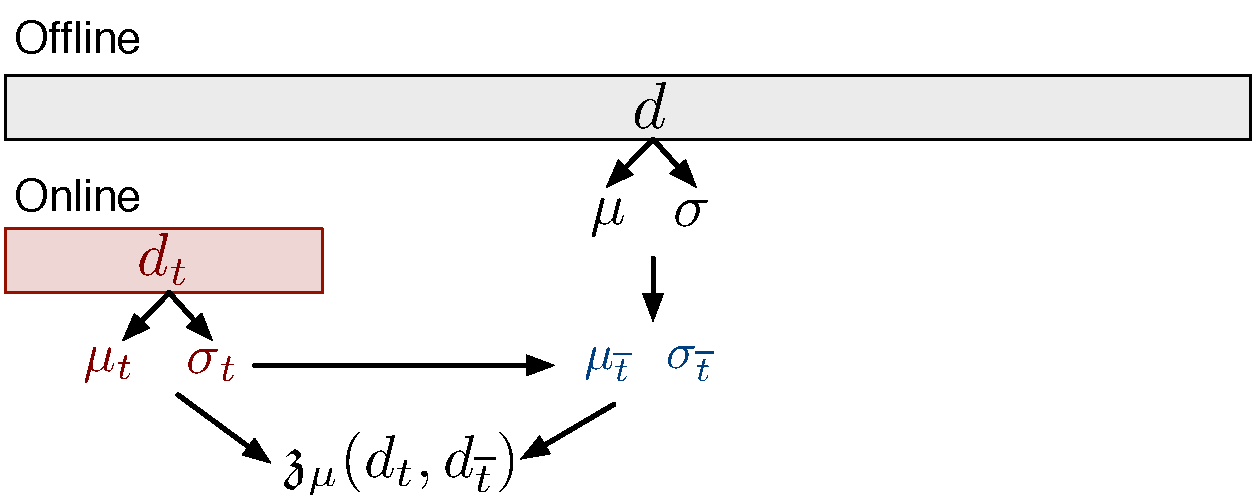
\includegraphics[width=\textwidth]{Figures/Staging2}
    \caption{Computing  $\mf{z}_\mu$  with staging.}
    \label{pic:withstag}
    \end{subfigure}
    \caption{Our staging strategy.}
\end{figure}


\subsection{Staging Computations}
\label{sec:optimization}
We now discuss how to compute the Zig-Components for each column of the
database. This task is critical: in the best case, it requires a full scan of
the database. In the worst case it runs in $\mathcal{O}(NM^2)$, because
we need to compute and compare every possible pair of correlations in
$\rb{V}_t$ and $\rb{V}_{\nott}$ for the scores $\mf{z}_r$ and $\mf{z}_V$.

Our idea is to prepare some computations offline, before the user starts
submitting queries.  Let us focus on the Zig-Component $\mf{z}_\mu$, which
reports the difference $(\bar{\bf{d}}_t - \bar{\bf{d}}_{\nott})/{s_{\nott}}$,
for a given column $\bf{d}$ of the database.  Figure~\ref{pic:withoutstag}
presents the naive method to compute this component.  As soon as our user
submits a selection, we compute the average $\bar{\bf{d}}_t$ for those tuples,
the values $\bar{\bf{d}}_{\nott}$ and $s_{\nott}$ for the rest of the database,
and we apply the formula $(\bar{\bf{d}}_t - \bar{\bf{d}}_{\nott})/{s_{\nott}}$
directly. Thus, we read the whole column.

Figure~\ref{pic:withstag} illustrates our staging strategy. Offline, we compute
the mean $\bar{\bf{d}}$ and the standard deviation $s$ for the whole
column~$\bf{d}$. Online, when the user submits a selection, we compute
$\bar{\bf{d}}_t$ and $s_t$
only - thus, we read the selection and ignore the rest of the database. We then
reconstitute $\bar{\bf{d}}_{\nott}$ and $s_{\nott}^2$, as follows:
\begin{gather}
    N_{\nott} = N - N_t\\
    \bar{\bf{d}}_{\nott}= \frac{ N \cdot \bar{\bf{d}} -  N_t \cdot \bar{\bf{d}}_t } { N - N_t } \\
    s_{\nott}^2 = \frac{N}{N_{\nott}} \cdot s^2 - \frac{N_t}{N_{\nott}} \cdot s_t^2 -
    \frac{N_t}{N} \cdot (\bar{\bf{d}}_t -  \bar{\bf{d}}_{\nott})^2 
\end{gather}
We now have all the elements to compute the Zig-Component. To obtain these
equations, we used formulas designed to compute the mean and variance
incrementally~\cite{pebay2008formulas}, and we reversed them - in fact we
compute $\bar{\bf{d}}_{\nott}$ and $s_{\nott}$ in a ``decremental'' fashion.

In effect, this method does not reduce the complexity of the algorithm, but it
greatly reduces the amount of tuples to read. The smaller the user's selection
is, the greater is the performance gain. Fortunately, we managed to extend it
for all the Zig-Components presented in Table~\ref{tab:dissim}.  We can derive
similar computations to update correlation
coefficients. If $q$ represents the covariance between $\bf{d}$ and $\bf{d}'$:
\begin{equation}
    q_{\nott} = \frac{N}{N_{\nott}} \cdot q - \frac{N_t}{N_{\nott}} \cdot q_t -
        \frac{N_t}{N} \cdot (\bar{\bf{d}}_t -  \bar{\bf{d}}_{\nott}) \cdot
                             (\bar{\bf{d}}'_t -  \bar{\bf{d}}'_{\nott}) 
\end{equation}
To cope with categorical data, our approach is slightly different. Offline, we
compute a histogram for $\bf{d}$.  Online we compute another histogram for
$\bf{d}_t$. From those, we can infer the distribution of $\bf{d}_{\nott}$'s
values, and compute $\mf{z}_\chi$ and $\mf{z}_V$.

\section{Model Validation}
\label{sec:validation}
We now focus on the following problem: for a given view $\rb{V}$, how
\emph{significant} is the Zig-Dissimilarity $D = \mf{D}( \rb{V}_t  ;
\rb{V}_{\overline{t}})$? A high value may indicate that $\rb{V}_t$ and
$\rb{V}_{\overline{t}}$ come from two different distributions.  But it could
also be caused by chance. How confident are we of this result? Answering this
question has two practical uses. First, a confidence score can help us decide
when to stop generating views. Second, it helps users interpret Ziggy's results.

The statistics literature proposes a completely ge\-ne\-ric way to solve
this problem: permutation testing. This methods works with the Zig-Dependency,
but it can also handle other divergence measures. The main idea is to
repeatedly shuffle the rows of $D^i$, without modifying $\rb{t}$. Thus, the
tuples are randomly affected to $\rb{V}_t$ and $\rb{V}_{\overline{t}}$. We
then observe how the dissimilarity $D$ varies: if the permutations have no
effect on $D$, then there is high chance that the dissimilarity was caused by
chance.  Oppositely, if $D$ is very sensitive,
then we have a high confidence in our result. We refer the interested
reader to Wasserman~\cite{wasserman2013all} for more details.

Permutation testing offers plenty of advantages, but shuffling the rows is
computationally heavy. In our implementation, we used an alternative approach.
The main idea is to use the composite nature of the Zig-Dissimilarity, and test
each Zig-Component individually. We then aggregate these scores in a synthetic
confidence indicator. Therefore we do not test the Zig-Dissimilarity directly -
instead we focus on its underlying effects.  This method is much lighter
because we can use known asymptotic results, or at least approximations
thereof. For instance, we know that under certain assumptions, we can test the
difference between the means with a Wald test~\cite{wasserman2013all}, which
only requires an extra $\mathcal{O}(1)$ computation.  Similarly, we can use a
F-test for the ratio of the variances, or a $\chi^2$ test for the differences
in categorical distributions.  Table~\ref{tab:tests} summarizes our choices. 
To aggregate the tests, we report the minimum observed confidence, an purposely
conservative approach~\cite{wasserman2013all}.

\section{Report Generation}
\label{sec:reporting}
\begin{figure}[t!]
  \centering
  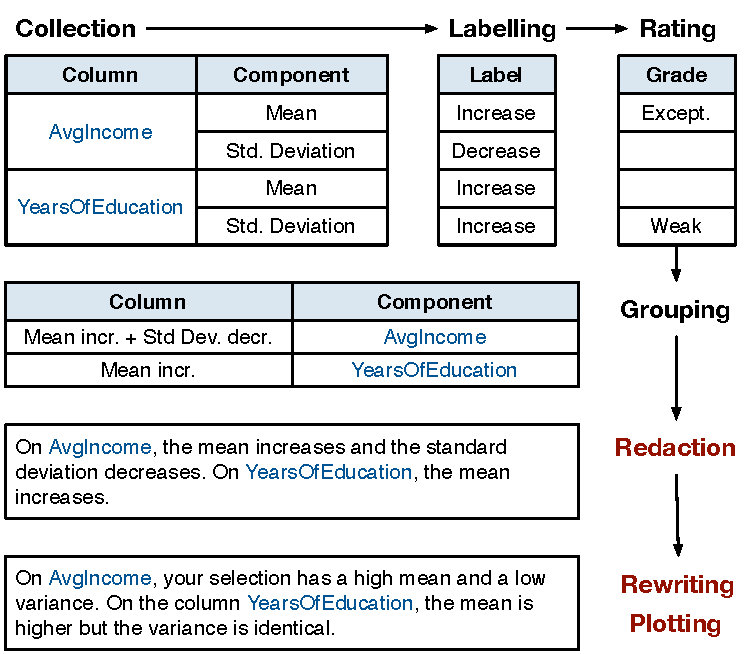
\includegraphics[width=0.95\columnwidth]{Figures/ReportGeneration}
  \caption{Ziggy's report generation pipeline.}
  \label{pic:reportpipeline}
\end{figure}
We explained how our system detects views. We now detail Ziggy's report generation
pipeline, through which it justifies its choices. 

Ziggy describes its views one by one. For each view, it generates a report,
comprising a few sentences and several charts. The aim of the text is to give a
general presentation of how the tuples differ from the rest of the data. The
charts let users inspect the details.  Figure~\ref{pic:reportpipeline}
illustrates how Ziggy proceeds. First, it gathers all the Zig-Components
associated with each columns of the database. It then generates a short
description for each component using hand-written rules such as those
presented in the first column of Table~\ref{tab:handwritten}. It also evaluates
each component, with a scale of three grades: ``weak'', ``neutral'', and
``exceptional''. These grades are based on both the values of the components
and their confidence, as illustrated in Table~\ref{tab:handwritten}.  To set
the thresholds, we took inspiration from classic statistics
textbooks~\cite{cohen1977statistical}, and chose conservative options.
Nevertheless, these quantities are inherently arbitrary. It is therefore
important to communicate them to the end users, and motivate each decision with
its corresponding rule.

Once Ziggy has collected, labeled and rated the Zig-Comp\-onents, it  groups
the columns which have the same ``profile'', that is, the same variations on
the same components. It then generates one sentence for each group, such that
each sentence has the same structure: \texttt{on [column\_names], the
[zig-component] [label]}. If several components are involved, as in
Figure~\ref{pic:reportpipeline}, the Ziggy enumerates all the pairs
\texttt{[zig-component] [label]}. At this point, the text produced is
understandable, but it is also highly redundant and possibly grammatically
incorrect. During the last phase, Ziggy rewrites the text a set of handwritten
rules. Such rules include inserting connectors (e.g., ``Additionally'',
``Finally''), using random synonyms (e.g., ``the tuples'', ``the selection'',
``your data'') or replacing wider chunks of text (e.g., ``has a lower
variance'' by ``spreads more widely'').

By default, Ziggy only produces visualizations for the variables associated
with exceptional components. It plots the remainder on demand. To determine
which type of visualization to use, it checks the type of the columns, and
applies usual techniques: it uses density plots and histograms for one
dimension data, and scatterplots and heat maps for two-dimension data.
\begin{table}[t!]
    \centering
    \begin{tabular}{| p{4cm} | c | c |}
      \hline
      Description & Exceptional? & Weak?\\
      \hline
      $\mf{z_\mu} \geq 0 \wedge \bar{\rb{d}}_{\nott} \geq 0$: ``increase'' &
          \multirow{4}{1.2cm}{$z_\mu^{\bf{d}}$ in top 5\%} & 
              \multirow{4}{1.5cm}{$|\mf{z_\mu^{\bf{d}}}| < 0.2$ or $p_\mu^{\bf{d}} < 0.01$}\\
      $\mf{z_\mu} \geq 0 \wedge \bar{\rb{d}}_{\nott} < 0$: ``decrease'' & &\\
      $\mf{z_\mu} < 0 \wedge \bar{\rb{d}}_{\nott} \geq0$: ``decrease'' & &\\
      $\mf{z_\mu} < 0 \wedge \bar{\rb{d}}_{\nott} < 0$: ``increase'' & &\\
      \hline
    \end{tabular}
    \caption{Example of handwritten rules for the difference of means
    $\mf{z_\mu}$. The variable $p_\mu$ describes the confidence (p-value), as
described in Section~\ref{sec:validation}.} 
\label{tab:handwritten}
\end{table}


\section{Setting Parameters}
\label{sec:parameters}

Ziggy's model relies on three parameters: the total number of views $K$ to
generate, the width of the views $D$, and the dependency threshold $L$. 

\textbf{Number of Views K.} When should we stop producing views? We propose to
generate as many views as possible, and delegate the final decision to the
users - after all, we have little idea about what they seeking. In practice, we
do so lazily: we start with a small selection of views (e.g., as many as
the display can contain), and we generate the remainder on demand, for instance
with a ``show me more'' button.  In our experience, the number of views stays
manageable because the algorithm is blocked by the redundancy constraint: after
a certain number of views, Ziggy finds no more columns to exploit. If the views
have a low confidence (as detailed in Section~\ref{sec:validation}), then Ziggy
issues a warning.

\textbf{Size of the Views D.} In our implementation, we set this parameter in an adaptive
fashion, using a method presented by Zhu and Ghodsi~\cite{zhu2006automatic}.
The main idea is the following. When building a view, we keep track of the
gains $\Delta\mf{D}_d$ induced by each column $d$.  We then detect change
points in the sequence (e.g., ``jumps'' or ``elbows'').  If we observe such a
behavior, we truncate the current view and start a new one.  The advantage of
this method is that $D$ can adapt to each subspace. However, it is
only a heuristic. Fortunately, inaccuracies have little consequence in
practice: if the dependency constraint is weak, then the excluded columns are
simply pushed to the next view.

\textbf{Dependency threshold L.} Admittedly, there is no optimal way to set
this parameter: it depends entirely on the user and the exploration context. By
default, we use $\mf{S}_{hard}$, and we limit to $L=0.99$. This setting
enforces that the views are non-overlapping, but it adds no other constraint -
we see this as a safe option.

\textbf{Zig-Components.} Previously, we proposed several Zig-Components, in
order to capture a wide range of effects. In practice, nothing forces to use
them all. For instance, a user interested in quick and concise results may
prefer to ignore the bivariate components.


\section{Use Case}
\label{sec:usecase}

\begin{table}[!t]
    \centering
    \small
    \begin{tabular}{p{4cm} c c c} 
        \hline
        \multirow{3}{*}{Columns}  & Except. & Weak  & \multirow{3}{*}{Score}\\
                                  & Comp.   & Comp.& \\
                                  & (\%)    & (\%)& \\
        \hline
        Patent\_applications\_p\_inhabitant & \multirow{3}{*}{83.3}
        &\multirow{3}{*}{0} & \multirow{3}{*}{25.4} \\
        PCT\_patent\_applications&&&\\
        Personal\_earnings &&&\\
        \hline
        Dwellings\_no\_basic\_facilities&
        \multirow{4}{*}{64.2} &\multirow{4}{*}{7.1} & \multirow{4}{*}{18.9} \\
        Educational\_attainment&&&\\
        Emp.\_work\_very\_long\_hours&&&\\
        Life\_expectancy&&&\\
        \hline
        Average\_hours\_worked&
        \multirow{4}{*}{50} &\multirow{4}{*}{42.2} & \multirow{4}{*}{12.4} \\
        Population\_growth\_rates&&&\\ 
        Working\_age\_population&&&\\
        Pop\_under\_the\_age\_of\_15&&&\\
        \hline
        Assault\_rate, Homicide\_rate &
        \multirow{2}{*}{77.7} &\multirow{2}{*}{11.1} & \multirow{2}{*}{12.1} \\
        Current\_\-account\_balance&&&\\
        \hline
        Export\_Pharmaceutical&
        \multirow{4}{*}{57.1} &\multirow{4}{*}{57.1} & \multirow{4}{*}{11.4} \\
        Incidence\_part\_time\_emp&&&\\ 
        Long\_term\_unemp&&&\\ 
        Production\_crude\_oil&&&\\ 
        \hline
        Air\_pollution, Job\_security&
        \multirow{2}{*}{77.7} &\multirow{2}{*}{11.1} & \multirow{2}{*}{10.1} \\
        Student\_skills&&&\\
        \hline
        Employment\_rate&
        \multirow{3}{*}{66.6} &\multirow{3}{*}{33.3} & \multirow{3}{*}{7.1} \\
        Total\_primary\_energy\_supply&&&\\ 
        Trade\_Balance.\_Pharmaceutical&&&\\ 
        \hline
        Triadic\_patent\_year&
        \multirow{2}{*}{28.5} &\multirow{2}{*}{75.5} & \multirow{2}{*}{6.2} \\
        Time\_devoted\_to\_leisure&&&\\ 
        \hline
        Renewable\_energy\_supply&
        \multirow{3}{*}{33.3} &\multirow{3}{*}{55.5} & \multirow{3}{*}{5.5} \\
        Voter\_turnout&&&\\ 
        Total\_tax\_revenue&&&\\ 
        \hline
        Consultation\_on\_rule\_making&
        \multirow{3}{*}{7.1} &\multirow{3}{*}{78.5} & \multirow{3}{*}{5.3} \\
        Implicit\_GDP\_Price\_Indices&&&\\
        Years\_in\_education&&&\\
        \hline
        Quality\_of\_support\_network&
        \multirow{2}{*}{33.3} &\multirow{2}{*}{55.5} & \multirow{2}{*}{4.5} \\
        Taxes\_on\_income\_and\_profits&&&\\
        \hline
        Value\_Added\_of\_Industry&
        \multirow{3}{*}{0} &\multirow{3}{*}{100} & \multirow{3}{*}{2.9} \\
        Exchange\_Rates&&&\\
        Gross\_Domestic\_Product&&&\\
        \hline
    \end{tabular}
    \caption{Detail of Ziggy's views, sorted by decreasing order of score. The
    two middle columns indicate the proportion of Zig-Components considered as
Exceptional and Weak.}
    \label{tab:ziggysviews}
\end{table}
\begin{figure*}[!ht]
  \centering
  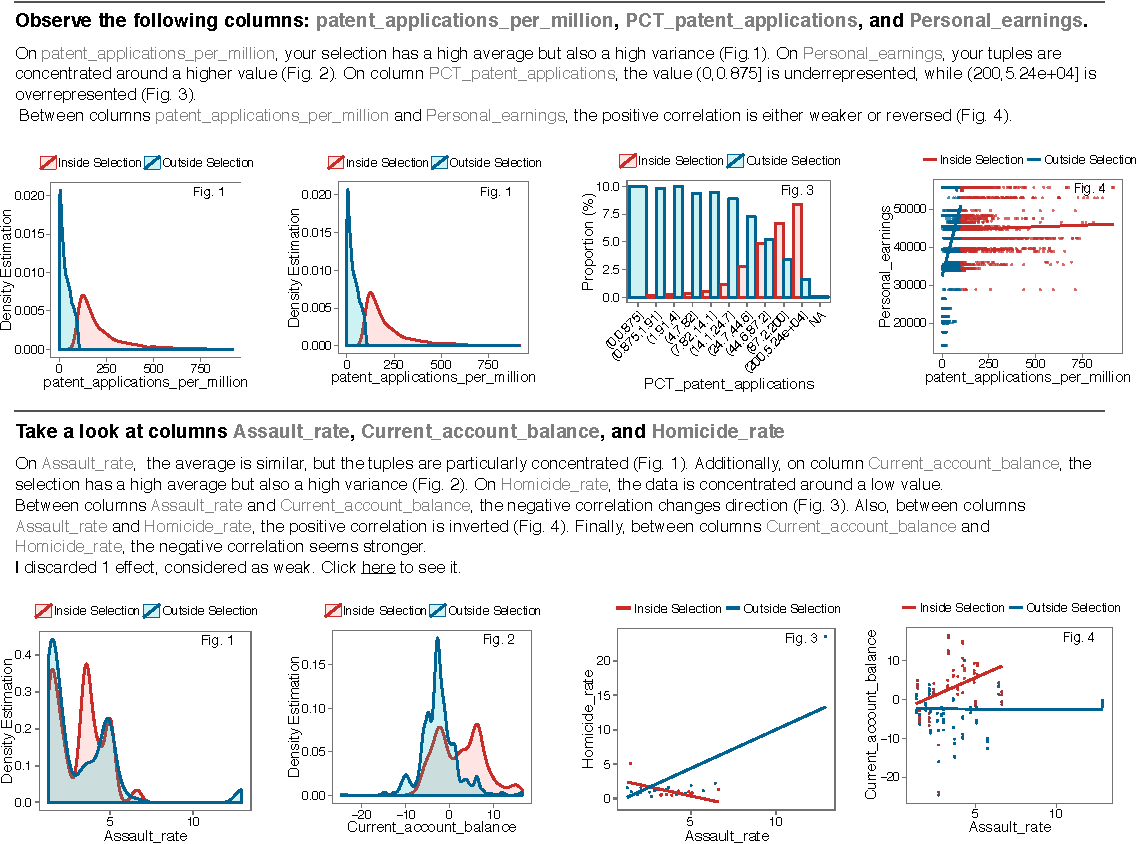
\includegraphics[width=2\columnwidth]{Figures/UseCase}
  \caption{Ziggy's explanations for Views 1 and 4}
  \label{pic:zigdetail}
\end{figure*}
We now apply Ziggy on the data which inspired our running example.
Our aim is to understand which factors lead to innovation, and more
specifically patents.  To answer this question, we aggregated several
databases from the OECD, an international economic organization. All the data
we used may be found online\footnote{http://stats.oecd.org/}. Our core dataset
is the \texttt{Patents per Region} database, which contains 15 years of patent
statistics for 2,180 regions in 31 countries. We augmented this set with
several other region-level databases (\texttt{Demo\-gra\-phics per Region} and
\texttt{Labour per Region}) and country-level indicators (\texttt{Better Life},
\texttt{Well Being} and \texttt{Innovation Indicators}).  We obtain a table
with about 6,823 rows and 519 columns, including mixed types and missing
values. We filtered out the categorical columns with more than 20 distinct
values (e.g., primary keys, countries and region names). 

Our selection of tuples contains the top 10\% regions for the statistic
\texttt{patent applications per inhabitant}. We set $D=6$, with the
adaptive stopping method described in Section~\ref{sec:parameters}. We use
$\mf{S}_{hard}$, with a maximum value of $L=0.75$.  Ziggy detects a total of 12
views, which columns are reported in Table~\ref{tab:ziggysviews}.

Some of Ziggy's choices are not surprising. For instance, the first
column mentioned in the Table is precisely the variable we used to define our
selection. The second one, $\texttt{PCT patent applications}$ is highly similar
(the PCT is an international patent treaty, which allows transnational
pa\-tents). Likewise, we expected some relationship between education and
innovation (views 2, 6 and 10). However, some effects are less straightforward.
How does \texttt{Employees working very long\- hours} impact innovation? Are
patents produced at work, or during hobby time? Similarly, how do our
innovative regions behave on the variable~\texttt{Job security}?

Figure~\ref{pic:zigdetail} presents Ziggy's explanations for two views. To
obtain this figure, we made only two edits: we removed some plots to save
space, and we inserted references to the charts in the text. Consequently, the
figure illustrates accurately what Ziggy's users would obtain. The first view
reflects the fact that innovative regions also have a high income. Ziggy
expresses this through its comments about the
variable~\texttt{Personal earnings}, but also through the last chart. As it
points out, there is a correlation between patent applications and income, but
this correlation disappears when we focus on innovative regions. Then, the
regression line is flat, with a high offset, which indicates that all these
regions are relatively rich, regardless of their patent statistics.

The second view offers a different perspective. The first and third charts show
that innovative regions tend to be safer, but the relationship is not
straightforward. Ziggy points out that these regions have less extreme values
on \texttt{Assault rate}, but the mean is similar. Also, the expected
correlation between \texttt{Assault rate} and \texttt{Homicide rate} is
inverted. This reflects the fact that assaults do exist in our innovative
regions, but little of them actually lead to a homicide. The last chart is more
puzzling: normally, there exists no relationship between \texttt{Assault rate}
and \texttt{Current ac\-count balance}. And indeed, we expect these variables
to be independent, because they describe completely different topics. Yet,
in the innovative regions, a clear correlation appears. How can we interpret
this effect? If this dependence completely spurious? Are those
variables cofounded by a third, hidden variable? Or maybe sane public accounts
causes anger among inventors? As implausible as this last hypothesis may seem, this
chart gives us no way to discard it. We leave the question open for future
investigations.

\section{Experiments}
\label{sec:experiments}

\textbf{Metrics.} We now present our experimental results. We evaluate
three aspects of our system: the \emph{quality} the views, their
\emph{diversity}, and Ziggy's \emph{runtime}. To evaluate the quality of the
views, we simulate users with statistical classifiers. We assume that if a
classifier can learn from a view, then so can a real user. Technically, we
materialize the user's selection into a vector $\rb{t} = (t_1, \ldots,
t_n)^\top$: $t_i=1$ if the tuple is chosen, 0 otherwise.  We then train a
classifier, using the view $\bf{V}$ as feature set and the user's selection
$\bf{t}$ as target. To obtain our quality score, 
we check if the classifier can accurately model the user's selection $\rb{t}$ with the
variables in $\bf{V}$. If so, we deduce that the selection has a
``peculiar'' structure in the subspace, and therefore the view contains
exploitable information. Oppositely, if the classifier cannot reconstruct the
user's selection, then either the classifier is poor, or the view contains no
information about the selection. We use a 5-Nearest Neighbor (5-NN) classifier,
and we report the F1 measure with 5 cross-validation (higher is better). We
chose the 5-NN algorithm for convenience: it is fast, and it gave
us good predictive performance. 

To measure diversity, we report the number of distinct columns used by the
views in the result set (higher is better). We measure runtime with the total
wall clock time, including preprocessing in Ziggy's case (lower is better).

\textbf{Baselines.} We compare Ziggy to four state-of-the-art subspace
detection methods from the data mining literature. Our first three methods are
supervised: their aim is to detect informative columns for a classification or
regression task.  We adapt these methods to our problem by setting $\bf{t}$ as
the target column. Here again, our rationale is the following: if a set of
column is a good predictor for the user's selection, then it contains useful
information.

Our first baseline is \texttt{Claude}~\cite{Sellam2015Semi}, a recently
published feature search algorithm. We chose this method because it uses a
multi-view approach, and therefore its results are directly comparable to ours:
like Ziggy, it returns a fixed number of subspaces, with a user-specified
number of dimensions.  Technically, Claude differs on two points. First, it
uses a different notion of interestingness: it seeks groups of columns which
are strongly dependent to the target, dependency being measured with the mutual
information. Second, Claude builds subspaces with a level-wise, beam search
algorithm. We used the authors' implementation.  We expect this approach to be
both fast and accurate.

Our second baseline is \texttt{Clique}, inspired by the pattern mining
literature~\cite{xie2010max}. The idea is to build a graph inside which the
weight of each edge $(i,j)$ represents the statistical dependency between the
pair of columns $i,j$ and the target variable (again, we measure dependency
with the mutual information) . To obtain $K$ subspaces with at most $N$
variables, we remove all the edges except the $K' > K$ strongest, and detect
cliques of at most $N$ nodes in the remaining graph. By default, we set $K' =
2\cdot K$. To detect cliques, we used the \texttt{igraph} software package. We
expect this algorithm to be fast but rather approximative.

Our third baseline, \texttt{Wrap-5NN} is a ``wrapper'' from the feature
selection literature~\cite{guyon2003introduction}. This algorithm trains 5-NN
classifiers with increasingly large sets of variables. First, it tests each
variable, and it keeps the top $K$. Then, it tests combinations of two columns.
The process is repeated until the views reach $D$ dimensions. We chose 5-NN
because it is the algorithm we use to evaluate the views. Therefore, we
optimize exactly what we measure. We expect this approach to be accurate, but
also very slow. Thus, we only use it as a ``gold standard'' for our experiments
with real data.

The last baseline, \texttt{4S}, detects subspaces in an unsupervised manner: it
seeks subspaces which contain clusters and outliers, independently of the
user's selection. To do so, it detects groups of variables which are strongly
mutually dependent, using an multivariate correlation measure. We used the
author's implementation written in Java. We expect $\texttt{4S}$ to be fast,
but also less accurate than its competitors because of it unsupervised nature.

\textbf{Setup.} We implemented Ziggy in R, exploiting its native primitives for critical
operations (namely computing means, covariance matrices and cross-tabulation).
We interrupted all the experiments which lasted more than 1 hour. Our test
system is based on a 3.40 GHz Intel(R) Core(TM) i7-2600 processor. It is
equipped with 16 GB RAM, but the Java heap space is limited to 8 GB. All the
algorithms we present are single-threaded. The operating system is Fedora 16.

\begin{figure*}[t!]
  \centering
  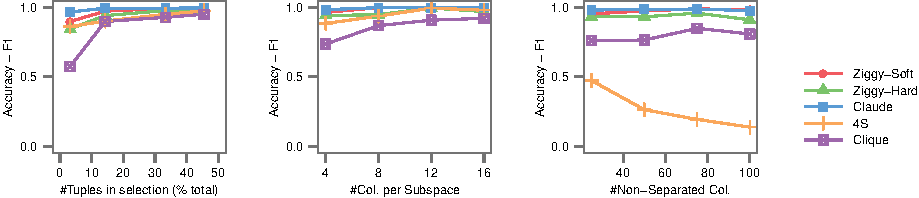
\includegraphics[height=3.5cm]{Plots/Synth-Accuracy}
  \caption{Average quality of the views varying the data generator parameters.}
  \label{pic:synthquali}
\end{figure*}
\begin{figure*}[t!]
    \centering
    \begin{subfigure}[b]{0.5\textwidth}
        \centering
    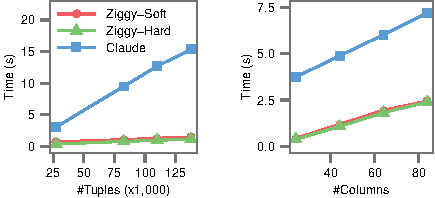
\includegraphics[height=3.5cm]{Plots/Synth-Runtime}
    \caption{Runtime for the three fastest algorithms, varying data parameters.
    The points for \texttt{Ziggy-Hard} and \texttt{Ziggy-Soft} overlap.}
    \label{pic:genruntime}
    \end{subfigure}
    ~~
    \begin{subfigure}[b]{0.45\textwidth}
        \centering
        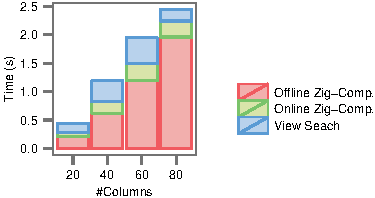
\includegraphics[height=3.5cm]{Plots/Synth-TimeDetail}
        \caption{Breakdown of the total runtime for \texttt{Ziggy-Soft},
        varying the number of columns.}
    \label{pic:detruntime}
    \end{subfigure}
  \label{pic:syntruntime}
    \caption{Runtime experiments with synthetic data.}
\end{figure*}

\begin{table}[t!]
    \centering
    \small
    \begin{tabularx}{\columnwidth}{X  c }
      \hline
      Parameter & Value\\
      \hline
      Selection (tuples) & 3,000\\
      Tuples from Gauss. mixture & 15,000\\ 
      Tuples from Unif. distrib. & 15,000\\
      Sep. / Non-sep. variables & 20 / 4\\
      \hline
      Num. dimensions subspaces & 4\\
      Num. components Gaussians& 5\\
      Mean / Variance Gaussians & Unif. in [-10,10] / [1, 20]\\
      Uniform noise & Unif. in [-45,45]\\
      \hline
    \end{tabularx}
    \caption{Default parameters for our data generator.} 
\label{tab:synthparameters}
\end{table}

\subsection{Synthetic Data}
\label{sec:synthexp}


In this set of experiments, we benchmark our algorithms in a synthetic
environment. Since we know the structure of the data in advance, we can tune
the competitors optimally. For instance, if we generate a dataset with 3
subspaces of 5 columns, then we set $K=3$ and $D=5$. We must however report
that \texttt{4S} tunes itself: it computes how many subspaces to generate, and
how large these should be. We use two versions of Ziggy: for
\texttt{Ziggy-Soft} we use the dependency measure $\mf{S}_{soft}$ and we limit
it to 0.1. For \texttt{Ziggy-Hard}, we use $\mf{S}_{hard}$ and we limit it
to~0.9.

Our generator produces columns by groups. It
yields two types of subspace: \emph{non-separated} subspaces, and
\emph{separated} subspaces. In the non-separated case, the selection and the
rest of the data are sampled from the same distribution, namely a mixture of
multivariate Gaussians with random parameters. In the separated case, the
selection is sampled from a separate Gaussian distribution, with its own random
parameters. Additionally, our generator produces uniform noise on all the
columns. Table~\ref{tab:synthparameters} presents our parameters. For each
experiment, we generate 4 random data sets and report the average F1 of all the
views.

\textbf{Quality of the Views.} The first chart in Figure~\ref{pic:synthquali}
presents the robustness of the algorithms with regards to the size of the
selection. For all our baselines, raising this parameter ameliorates the views, 
but the quality converges fast (at around 15\% of the database size).  The
algorithm \texttt{Claude} comes first, but it is very closely followed by the
two instances of \texttt{Ziggy} and \texttt{4S}. The ranking is almost
identical in the second chart, which displays the accuracy of the algorithms
varying the dimensionality of the subspaces. All algorithms involved seem
robust, but \texttt{Ziggy-Soft}, \texttt{Ziggy-Hard} and \texttt{Claude}
are above, followed closely by \texttt{4S}, then
\texttt{Clique}. The last graph illustrates the robustness of the views with
regards to the number of non-separated columns.  All our baselines achieve good
scores, except \texttt{4S}. We interpret this effect by the fact that
\texttt{4S} is unsupervised, it has therefore now way to detect which subspaces
are interesting and which are not. In conclusion, despite its simple
assumptions, Ziggy delivers high quality, robust views, largely comparable to
state-of-the-art feature selection algorithms.

\textbf{Runtime.} Figure~\ref{pic:genruntime} illustrates the total runtime
with regards to the number of rows and columns in the database. We ignored the
algorithms \texttt{4S} and \texttt{Clique}, which were slower than the other
candidates. We observe that Ziggy's performance is spectacular: it is an order
of magnitude faster than \texttt{Claude}, which is itself faster than the other
competitors. And yet, all the algorithms involved in our benchmark have the
same $\mathcal{O}(ND^2)$ complexity. We explain the difference with Ziggy's
simpler computations. Ziggy relies on means and correlations, which are much
lighter than \texttt{Claude}'s information theoretic estimators. Besides, when
evaluating its views, Ziggy considers at most two dimensions at a time, while
its competitors test higher level dependencies.

Figure~\ref{pic:detruntime} shows where \texttt{Ziggy-Soft} spends its time.
By far, the most expensive operations are the offline computations. This
validates our staging strategy.  Table~\ref{tab:synthparameters} reports that
the database contains 1 selected tuple for every 10 non selected tuple.
Therefore we expected the online phase to be about 10 times faster, ignoring
overhead costs. The figure confirms this estimation.

\textbf{Diversity.} Figure~\ref{pic:synthvariety} presents the number of
distinct co\-lumns mentioned in the views. In the leftmost chart, we compare
four competitors, varying the width of the subspaces. We notice two distinct
groups of columns. The approaches \texttt{Ziggy-Hard} and \texttt{4S} offer a
very high diversity, because they enforce that no columns is shared among
subspaces. The approaches \texttt{Claude} and \texttt{Ziggy-Soft} offer much
less variety. The rightmost figure illustrates the effect of the dependency
threshold. In the Hard case, it has no apparent effect because the views are
completely disjoint anyway (the threshold  does separate the correlated
columns, but this does not influence our metric). In the Soft case, we see that
our deduplication strategy works" a lower threshold forces Ziggy to introduce
variety.

\begin{figure}[t!]
  \centering
  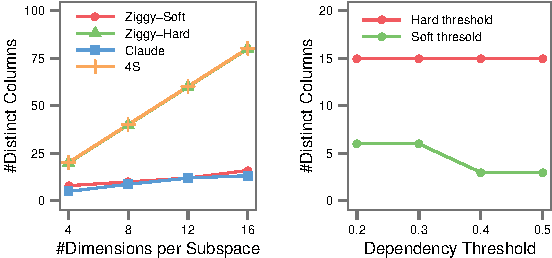
\includegraphics[height=3.5cm]{Plots/Synth-Dedup}
  \caption{Variety of the views.}
  \label{pic:synthvariety}
\end{figure}

\subsection{Real Data}
\label{sec:realdata}

\begin{figure*}[!ht]
  \centering
  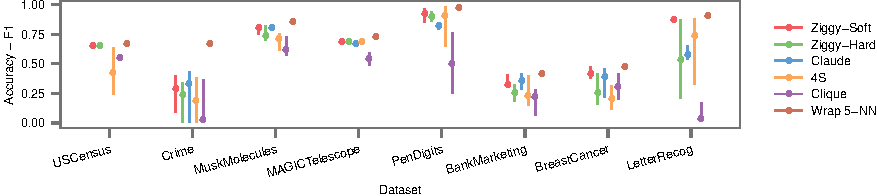
\includegraphics[width=0.8\textwidth]{Plots/Real-Accuracy}
  \caption{Quality of the views. The points represent median scores, the bars
  represent the lowest and greatest scores.}
  \label{pic:realquali}
\end{figure*}
\begin{figure*}[!ht]
  \centering
  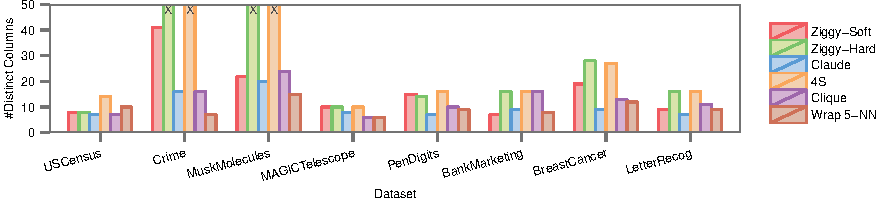
\includegraphics[width=0.8\textwidth]{Plots/Real-Diversity}
  \caption{Diversity of the views. The \texttt{X} mark indicates that we 
  truncated the column.}
  \label{pic:realdiversity}
\end{figure*}
\begin{figure*}[!ht]
  \centering
  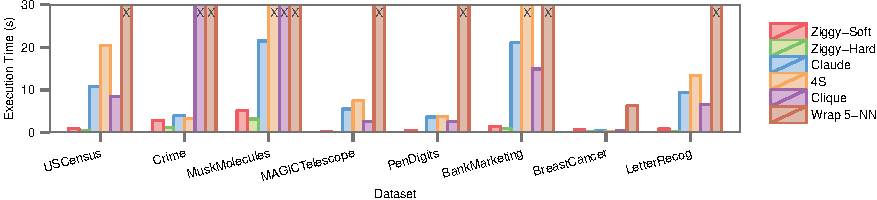
\includegraphics[width=0.8\textwidth]{Plots/Real-Runtime}
  \caption{Runtime. The \texttt{X} mark indicates that we truncated the column.}
  \label{pic:realruntime}
\end{figure*}
We now presents our experiments on real data from the UCI Repository. We
introduce the algorithm \texttt{Wrap-5NN}, which we use as ``gold standard'',
since it optimizes precisely the metric we report. To set the number and width
of the subspaces, we rely on \texttt{4S}. Table~\ref{tab:datasets} describes the
datasets and our settings. Because all the competitors have the same
parameters, the comparison is fair.

\textbf{Accuracy.} Figure~\ref{pic:realquali} illustrates the quality of the
views for each algorithm. We observe that \texttt{Wrap 5-NN} comes always
first. It is followed by \texttt{Ziggy-Soft},\texttt{Claude} and
\texttt{Ziggy-Hard}, often closely (although \texttt{Crime} is a striking
counter-example) and in different orders. The unsupervised
\texttt{4S} follows in most cases, tailed by \texttt{Clique}. Here again, we
conclude that Ziggy's performance is largely comparable to good feature
selection algorithms. However, we observe that \texttt{Ziggy-Hard} is often
below \texttt{Ziggy-Soft}, the most extreme case being the \texttt{LetterRecog}
set.  This is a consequence of its diversity. In the synthetic case, Ziggy had
several equally good subspaces to chose from. In the last three datasets, it
seems that some subspaces are better than others, and therefore non-redundancy
induces an accuracy loss (observe that \texttt{4S} suffers from the same
problem).

\textbf{Diversity.} Figure~\ref{pic:realdiversity} presents the diversity
results.  As with synthetic data, we observe that \texttt{4S} and
\texttt{Ziggy-Hard} dominate the other algorithms, in particular with wide
datasets such as \texttt{Crime} and \texttt{MuskMolecules}. The algorithms
\texttt{Ziggy-Soft} and \texttt{Clique} follow, then \texttt{Claude} and
\texttt{Wrap-5NN} comes last - which we expected since they mostly target
accuracy. This chart, in conjunction with Figure~\ref{pic:realquali}, shows
that the algorithms which generate the best F1 rarely generate the best
diversity, and reciprocally. This motivates our choice to offer both
$\mf{S}_{Hard}$ and $\mf{S}_{Soft}$.

\textbf{Runtime} We present the runtime of our algorithms in
Figure~\ref{pic:realruntime}. The results are consistent with our previous
conclusions: Ziggy outperforms all of its competitors, and the speedup gets more
dramatic as the size of the datasets increase.

\begin{table}[!t]
    \centering
    \small
    \begin{tabular}{r c c c c} 
        \hline
        Dataset & Columns & Rows & \#Views & Dim Views\\
        \hline
        MuskMolecules & 167 & 6,600 & 22 & 18\\
        Crime & 128 & 1,996 & 20 & 17\\
        BreastCancer & 34 & 234 & 10 & 13\\
        PenDigits & 17 & 7,496 & 9 & 10\\
        BankMarketing & 17 & 45,213 & 11& 8\\
        LetterRecog & 16 & 20,000 & 10 & 12\\
        USCensus & 14 & 32,578 & 10 & 7\\
        MAGICTelescope & 11 & 19,022 & 1 & 10\\
        \hline
    \end{tabular}
    \caption{Characteristics of the datasets.}
    \label{tab:datasets}
\end{table}

\section{Related Work}
\label{sec:related-works}

\textbf{Outlier Description.} Outlier description consists in finding subspaces
inside which a particular tuple is an outlier~\cite{angiulli2009detecting,
duan2014mining,knorr1999finding,zhang2006detecting}. This task inspired our
work, but its objectives are different. Outlier description describes single
objects, while we describe sets of tuples.  It focuses on distance-based
outliers, while we focus on probability distributions, regardless of how
central or isolated the user's selection is.  Authors focus on specific data
types (either numerical or categorical, but not both), and little of them
mention redundancy (an exception is~\cite{duan2014mining}, which seeks closed
sets). None of these works discuss how to report results.

\textbf{Contrast Mining.} Contrast mining is a similar task, but in a pattern
mining context: the aim is to differentiate two or more populations by
identifying patterns which are present (e.g., have a high support) in one
population and not the
other~\cite{vreeken2007characterising,webb2008detecting}. This line of work is
related but orthogonal, because we deal with neither itemsets nor patterns.
Notably, Loekito and Bailey introduced a  method to identify discriminative 
variables~\cite{loekito2008mining}.  Yet, their work focus on ``contrast of
contrasts'' for categorical data, a close but different task

\textbf{Feature Selection.} As noted in Section~\ref{sec:experiments}, our work
is intimately related to feature selection. Feature selection seeks predictive
variables for a classification or regression task~\cite{guyon2003introduction}.
We can map this task to our problem by treating the user's selection as a
column to be predicted. The main difference is that feature selection seeks
statistical accuracy, while we target interpretation. Thus, most feature
selection algorithms seek one optimal set of variables, while we seek several
small sets of variables. Also, they optimize class separability,
while we are interested in any difference in distribution. Nevertheless, we
acknowledge the similarity between our work and some feature selection
algorithms, and compare them directly in Section~\ref{sec:experiments}.

\textbf{Data Exploration} Recent works in data exploration have tackled
different but related problems. Similarly to our work,
SeeDB~\cite{vartak2015see} re\-com\-mends visualizations by seeking co\-lumns on
which a set of tuples have an unusual behavior. However, they focus on
\texttt{GROUP BY} aggregates on data warehouses, while we focus on
statistical descriptors on flat tables. Lloyd et al.'s automated
statistician~\cite{Lloyd2014ABCD} describes regression models in natural
language. These approaches are somewhat complementary to ours, and there would
be much to gain by combining them.


\section{Conclusion}
\label{sec:conclusions}
We exposed the tuple characterization problem, and presented our solution,
Ziggy. Our experiments show that Ziggy can produce informative, non-redundant
results within a fraction of the time taken by state-of-the-art machine
learning algorithms. In fact,  we could apply our solution to a wide range of
problems beyond the strict realm of data exploration, including feature
selection and subspace search.

We are genuinely excited by the perspectives offered by our results. In the
future, we will study how our system can adapt to the user's preferences. We
will investigate to what extent we can enrich our framework with other measures
of difference, using for instance Bayesian modeling. Finally, the problem of
how to describe tuples with natural language is immense, but it has, to the
best of our knowledge, only received little attention. We believe that this
field is full of promises, for data explorers and data researchers alike.


%\section*{[Private] Appendix: Ziggy vs.Claude}
%\label{zigvsclaude}
%We may now wonder: if we set $\mf{D}$ as the KL divergence, what is the
%difference between Claude and Ziggy?  Suppose that we ignore the penalty factor
%(we set $\lambda=0$). Then Ziggy tries to maximize:
%$$
%KL\big(\rb{x} | t=0 \ ; \  \rb{x} | t=1 \big)
%$$
%Intuitively, this is the distance between $\rb{x} | t=0$ and $\rb{x} | t=1$.
%On the other hand, Claude maximizes $I(\rb{x}, t)$. With a bit of playinFirst, look at columns AvgIncome and YearsOfEducation. Observe that the mean….g
%around, we can show that this is equivalent to maximizing:
%$$
%    KL\big(\rb{x} | t=0 \ ; \  \rb{x} \big) + 
%        KL\big(\rb{x} | t=1 \ ; \  \rb{x} \big)
%$$
%Here, we are interested in the distance between $\rb{x} | t=i$ and a central
%distribution $\rb{x}$. 
%
%There is a triangular relationship between these expressions:
%\begin{figure}[h!]
%  \centering
%  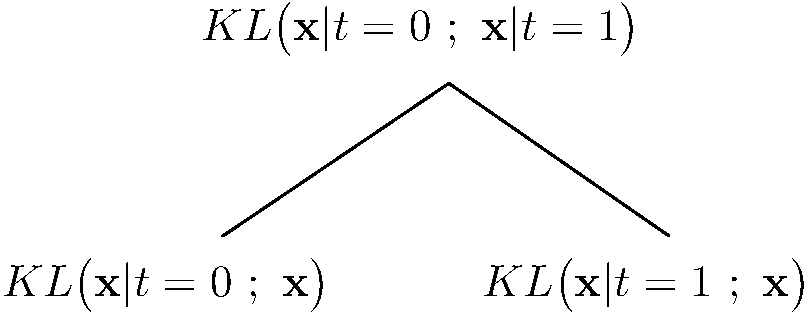
\includegraphics[width=0.6\columnwidth]{Figures/Triangle}
%  \label{pic:triangle}
%\end{figure}
%
%I wonder if they are not actually equivalent!


